\documentclass[border=5pt,multi]{standalone}
\usepackage{tikz}
\usepackage{filecontents}
\usepackage{gitdags}

\usepackage{xcolor}
\usepackage{listings}

\definecolor{ForestGreen}{rgb}{0.1,1.0,0.1}
\definecolor{Dandelion}{rgb}{0.9412,0.8824,0.1882}
\definecolor{Red}{rgb}{1.0,0.0,0.0}
 

% gitgraph.txt contains raw output of: $ git log --graph --oneline
\begin{filecontents}{gitgraph.txt}
* d764b48 added plaintext version in markdown
* 54ba4b2 release 2014-01-25
*   c589395 Merge branch 'master'
|\
| * 9f9c652 Remove holdover from kjh gh-pages branch
* | b3bd158 exclude font files
|/
* 63268c1 micro-typography
\end{filecontents}

\newcommand\commit[2]{\node[commit] (#1) {}; \node[clabel] at (#1) {\texttt{#1}: #2};}
\newcommand\ghost[1]{\coordinate (#1);}
\newcommand\connect[2]{\path (#1) to[out=90,in=-90] (#2);}

\begin{document}

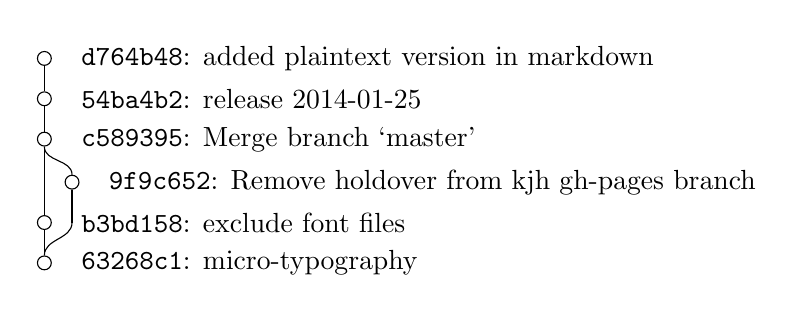
\begin{tikzpicture}
    \tikzstyle{commit}=[draw,circle,fill=white,inner sep=0pt,minimum size=5pt]
    \tikzstyle{clabel}=[right,outer sep=1em]
    \tikzstyle{every path}=[draw]
    \matrix [column sep={1em,between origins},row sep=\lineskip]
    {
        % Row 1
        \commit{d764b48}{added plaintext version in markdown}  % 1-1
        & 
        \\

        % Row 2
        \commit{54ba4b2}{release 2014-01-25}  % 2-1
        & 
        \\

        % Row 3
        \commit{c589395}{Merge branch `master'} % 3-1
        & 
        \\

        % Row 4
        & 
        \commit{9f9c652}{Remove holdover from kjh gh-pages branch}  % 4-2
        \\

        % Row 5
        \commit{b3bd158}{exclude font files}  % 5-1
        & 
        \ghost{branch1}  % 5-2
        \\

        % Row 6
        \commit{63268c1}{micro-typography} % 6-1
        & 
        \\
    };
    \connect{63268c1}{b3bd158};
    \connect{63268c1}{branch1};
    \connect{branch1}{9f9c652};
    \connect{b3bd158}{c589395};
    \connect{9f9c652}{c589395};
    \connect{c589395}{54ba4b2};
    \connect{54ba4b2}{d764b48};
\end{tikzpicture}

\vspace{10em}

\begin{tikzpicture}
      % Commit DAG
      \gitDAG[grow right sep = 2em]{
        A -- B -- { 
          C,
          D -- E,
        }
      };
      % Tag reference
      \gittag
        [v0p1]       % node name
        {v0.1}       % node text
        {above=of A} % node placement
        {A}          % target
      % Remote branch
      \gitremotebranch
        [origmaster]    % node name
        {origin/master} % node text
        {above=of C}    % node placement
        {C}             % target
      % Branch
      \gitbranch
        {master}     % node name and text 
        {above=of E} % node placement
        {E}          % target
      % HEAD reference
      \gitHEAD
        {above=of master} % node placement
        {master}          % target
\end{tikzpicture}

\vspace{10em}

\begin{tikzpicture}
      \gitDAG[grow right sep = 2em]{
        A -- B -- { 
          C -- D' -- E',
          {[nodes=unreachable] D -- E },
        }
      };
      % Tag reference
      \gittag
        [v0p1]       % node name
        {v0.1}       % node text
        {above=of A} % node placement
        {A}          % target
      % Remote branch
      \gitremotebranch
        [origmaster]    % node name
        {origin/master} % node text
        {above=of C}    % node placement
        {C}             % target
      % Branch
      \gitbranch
        {master}      % node name and text 
        {above=of E'} % node placement
        {E'}          % target
      % HEAD reference
      \gitHEAD
        {above=of master} % node placement
        {master}          % target
      \SAandWT
\end{tikzpicture}

\vspace{10em}

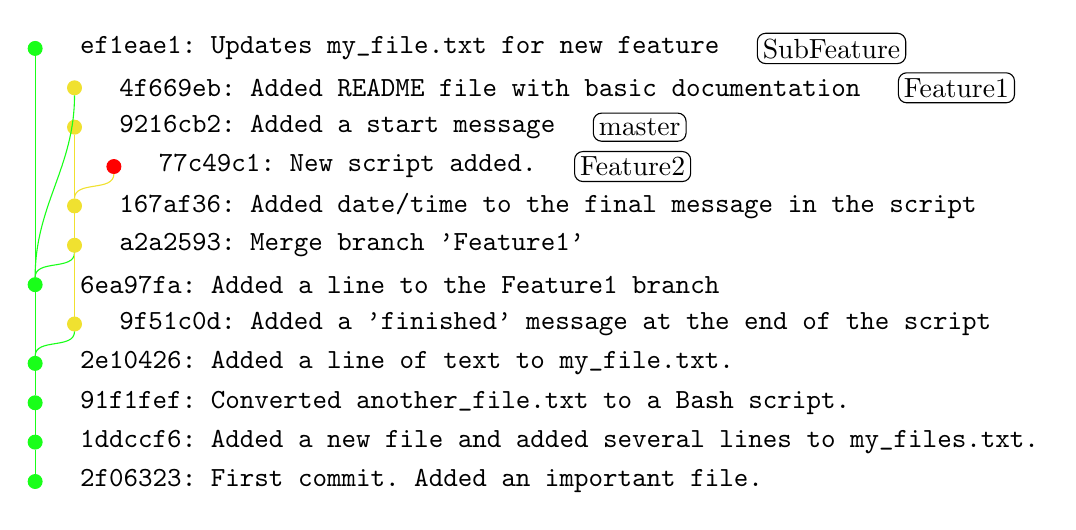
\begin{tikzpicture}
    \tikzstyle{commit}=[draw,circle,fill=white,inner sep=0pt,minimum size=5pt]
    \tikzstyle{every path}=[draw]
    \tikzstyle{branch}=[draw,rectangle,rounded corners=3,fill=white,inner sep=2pt,minimum size=5pt]
    \node[commit, ForestGreen, fill=ForestGreen] (ef1eae1) at (0.0,0) {};
    \node[right,xshift=10] (label_ef1eae1) at (ef1eae1.east) {\verb!ef1eae1: Updates my_file.txt for new feature!};
    \node[commit, Dandelion, fill=Dandelion] (4f669eb) at (0.5,-0.5) {};
    \node[right,xshift=10] (label_4f669eb) at (4f669eb.east) {\verb!4f669eb: Added README file with basic documentation!};
    \node[commit, Dandelion, fill=Dandelion] (9216cb2) at (0.5,-1.0) {};
    \node[right,xshift=10] (label_9216cb2) at (9216cb2.east) {\verb!9216cb2: Added a start message!};
    \node[commit, Red, fill=Red] (77c49c1) at (1.0,-1.5) {};
    \node[right,xshift=10] (label_77c49c1) at (77c49c1.east) {\verb!77c49c1: New script added.!};
    \node[commit, Dandelion, fill=Dandelion] (167af36) at (0.5,-2.0) {};
    \node[right,xshift=10] (label_167af36) at (167af36.east) {\verb!167af36: Added date/time to the final message in the script!};
    \path[Dandelion] (167af36) to[out=90,in=-90] (9216cb2);
    \path[Dandelion] (167af36) to[out=90,in=-90] (77c49c1);
    \node[commit, Dandelion, fill=Dandelion] (a2a2593) at (0.5,-2.5) {};
    \node[right,xshift=10] (label_a2a2593) at (a2a2593.east) {\verb!a2a2593: Merge branch 'Feature1'!};
    \path[Dandelion] (a2a2593) to[out=90,in=-90] (167af36);
    \node[commit, ForestGreen, fill=ForestGreen] (6ea97fa) at (0.0,-3.0) {};
    \node[right,xshift=10] (label_6ea97fa) at (6ea97fa.east) {\verb!6ea97fa: Added a line to the Feature1 branch!};
    \path[ForestGreen] (6ea97fa) to[out=90,in=-90] (ef1eae1);
    \path[ForestGreen] (6ea97fa) to[out=90,in=-90] (4f669eb);
    \path[ForestGreen] (6ea97fa) to[out=90,in=-90] (a2a2593);
    \node[commit, Dandelion, fill=Dandelion] (9f51c0d) at (0.5,-3.5) {};
    \node[right,xshift=10] (label_9f51c0d) at (9f51c0d.east) {\verb!9f51c0d: Added a 'finished' message at the end of the script!};
    \path[Dandelion] (9f51c0d) to[out=90,in=-90] (a2a2593);
    \node[commit, ForestGreen, fill=ForestGreen] (2e10426) at (0.0,-4.0) {};
    \node[right,xshift=10] (label_2e10426) at (2e10426.east) {\verb!2e10426: Added a line of text to my_file.txt.!};
    \path[ForestGreen] (2e10426) to[out=90,in=-90] (6ea97fa);
    \path[ForestGreen] (2e10426) to[out=90,in=-90] (9f51c0d);
    \node[commit, ForestGreen, fill=ForestGreen] (91f1fef) at (0.0,-4.5) {};
    \node[right,xshift=10] (label_91f1fef) at (91f1fef.east) {\verb!91f1fef: Converted another_file.txt to a Bash script.!};
    \path[ForestGreen] (91f1fef) to[out=90,in=-90] (2e10426);
    \node[commit, ForestGreen, fill=ForestGreen] (1ddccf6) at (0.0,-5.0) {};
    \node[right,xshift=10] (label_1ddccf6) at (1ddccf6.east) {\verb!1ddccf6: Added a new file and added several lines to my_files.txt.!};
    \path[ForestGreen] (1ddccf6) to[out=90,in=-90] (91f1fef);
    \node[commit, ForestGreen, fill=ForestGreen] (2f06323) at (0.0,-5.5) {};
    \node[right,xshift=10] (label_2f06323) at (2f06323.east) {\verb!2f06323: First commit. Added an important file.!};
    \path[ForestGreen] (2f06323) to[out=90,in=-90] (1ddccf6);
    \node[branch,right,xshift=10] (Feature1) at (label_4f669eb.east) {\lstinline{Feature1}};
    \node[branch,right,xshift=10] (Feature2) at (label_77c49c1.east) {\lstinline{Feature2}};
    \node[branch,right,xshift=10] (SubFeature) at (label_ef1eae1.east) {\lstinline{SubFeature}};
    \node[branch,right,xshift=10] (master) at (label_9216cb2.east) {\lstinline{master}};
\end{tikzpicture}

\end{document}
